\section{Interfejs użytkownika}

W dzisiejszych czasach interfejs użytkownika graficzny użytkownika stanowi niezwykle istotny element każdego systemu
informatycznego. Powinien on łączyć w~sobie dwie cechy: użyteczność i~atrakcyjność. Ważne jest uzyskanie odpowiedniego
balansu pomiędzy tymi cechami. Skupienie się wyłącznie na użyteczności prawdopodobnie odbije się negatywnie na
atrakcyjności i~odwrotnie. 

Dodatkowo interfejs powinien nawiązywać do aktualnych trendów w~tej dziedzinie. Nawet najładniejsza i~łatwa w~obsłudze
aplikacja, która powstała kilka lat temu nie będzie dorównywała aplikacjom stworzonym na przestrzeni ostatnich miesięcy.
Wynika to głównie ze zmiany podejścia do tworzenia interfejsów. Obecnie projektowane interfejsy muszą często dobrze
przezentować się zarówno na komputerach stacjonarnych, jak i~urządzeniach mobilnych. Wymusza to stosowanie prostych
kontrolek, oraz ograniczanie ilości informacji do niezbędnych dla działania.

Obecny trend wskazuje, że za najładniejsze uznawane są aplikacje minimalistyczne (np.  material design). Przedstawiony
poniżej prototyp interfejsu został stworzony z~myślą o~użyteczności, jednak również jego atrakcyjność można uznać za
nawiązującą do panującej mody.

Należy pamiętać, że jest to jedynie prototyp i~nie prezentuje on wszystkich funkcjonalności, ani widoków jakie będzie
posiadał przyszły system, a~jedynie narzuca pewną konwencje, która powinna zostać zachowana przy tworzeniu pozostałych
elementów.

\newpage

\begin{figure}[H]
  \centering
  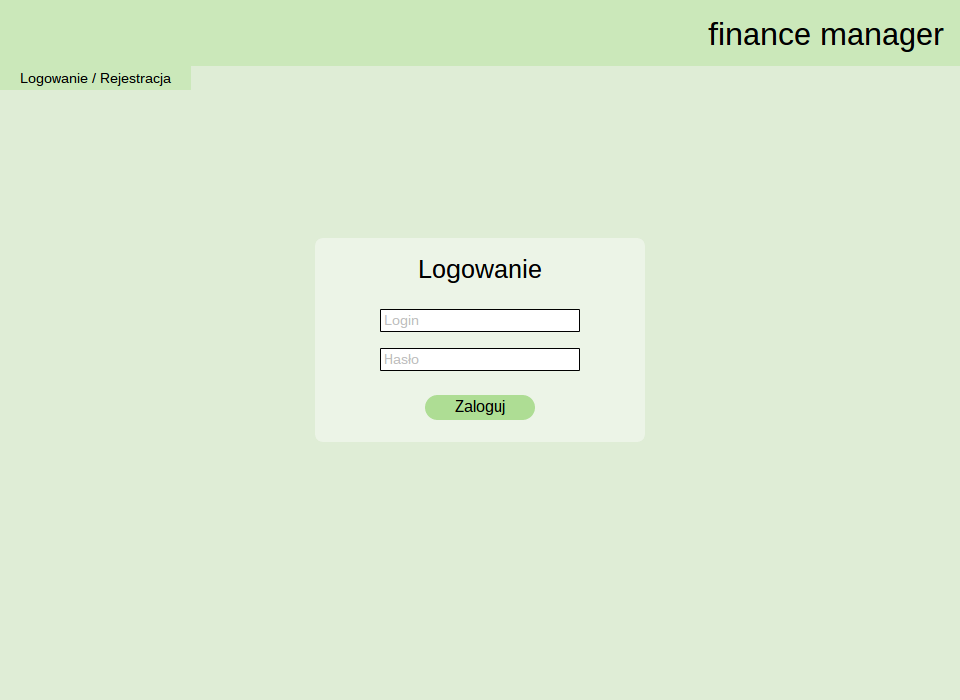
\includegraphics[width=\textwidth]{images/ui-login.png}
  \caption{Prototyp widoku logowania.}
  \label{pic:login}
\end{figure}

Strona startowa jaką zobaczy użytkownik prezentuje się jak na rysunku \ref{pic:login}. Z~tego poziomu każdy użytkownik
posiadający w~systemie konto będzie mógł zalogować się do swojego prywatnego panelu. Jeżeli system odwiedzi użytkownik,
który swojego konta w~systemie nie posiada, będzie on musiał przejść do strony rejestracji, klikając odpowiedni odnośnik
na banerze znajdującym się pod logo aplikacji.


\begin{figure}[H]
  \centering
  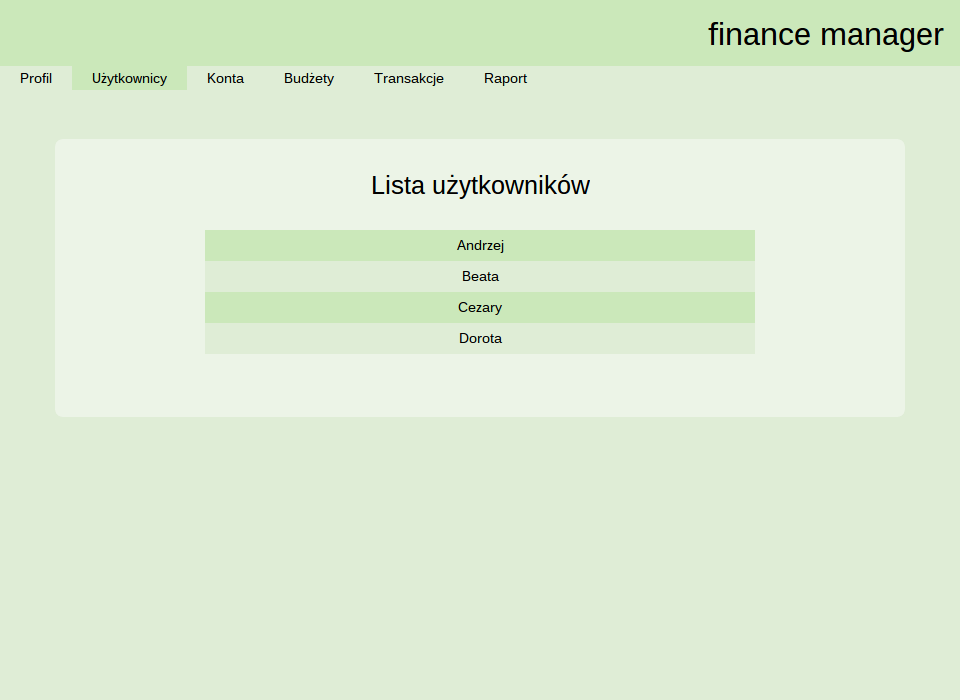
\includegraphics[width=\textwidth]{images/ui-user-list.png}
  \caption{Prototyp widoku z~listą użytkowników.}
  \label{pic:user_list}
\end{figure}

Wszystkie pozostałe prezentowane widoki zakładają, że użytkownik pomyślnie zalogował się do systemu. Na rysunku
\ref{pic:user_list} znajduje się widok z~listą użytkowników, tak aby każdy mógł sprawdzić, kto również posiada konto w
systemie.

\begin{figure}[H]
  \centering
  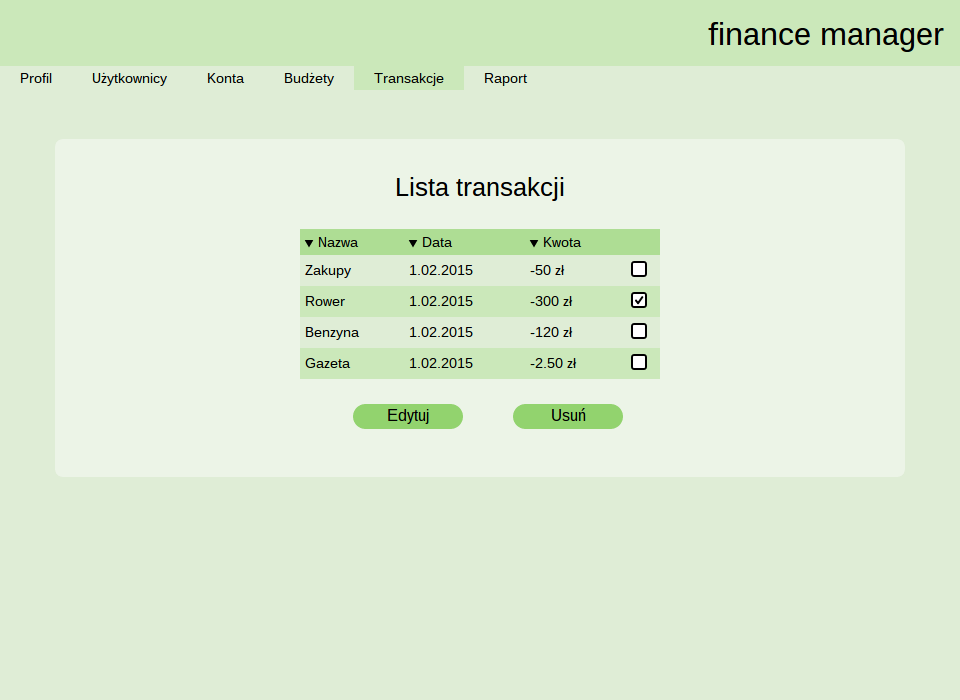
\includegraphics[width=\textwidth]{images/ui-trans.png}
  \caption{Prototyp widoku z~listą transakcji.}
  \label{pic:trans}
\end{figure}

Rysunek \ref{pic:trans} prezentuje widok transakcji. Z~tego poziomu użytkownik może dokonywać przeglądu dokonanych
wydatków, lub uzyskanych przychodów. Po zaznaczeniu odpowiedniej transakcji, uaktywniają się opcje edycji i~usuwania
zaznaczonej transakcji. Dzięki temu można kontrolować przypadkowo wstawione operacje, lub takie które nie mają
znaczącego wpływu na stan konta. Dodakowo, co może się okazać szczególnie przydatne w~przypadku gdy lista transakcji
urośnie do większych rozmiarów, istnieje możliwość sortowania transakcji według jednego z~trzech kluczy.

\begin{figure}[H]
  \centering
  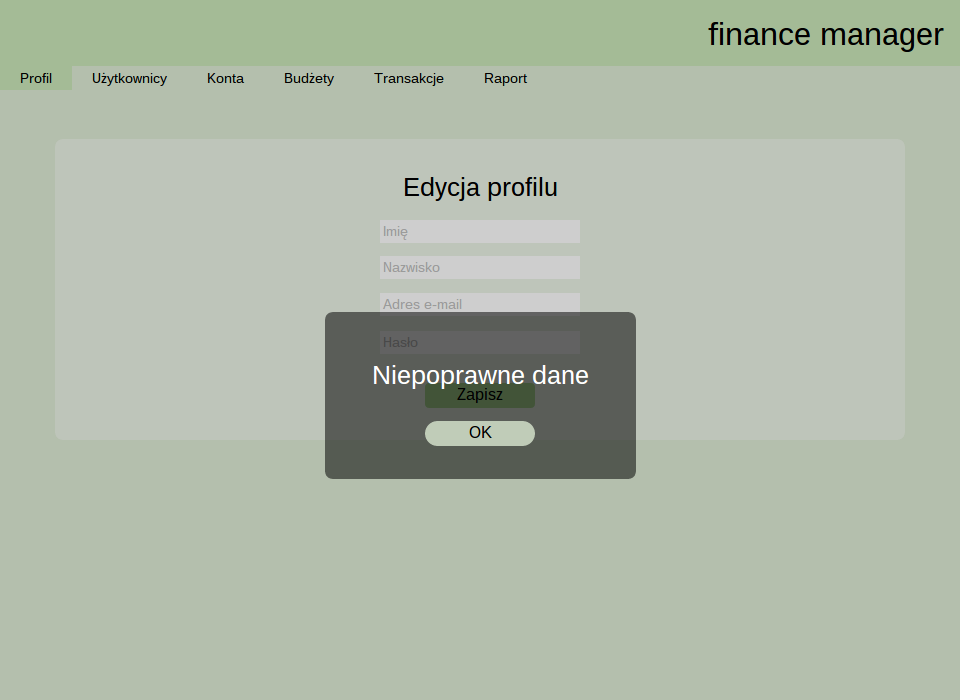
\includegraphics[width=\textwidth]{images/ui-profile-edit-err.png}
  \caption{Prototyp widoku pozwalającego na edycję danych użytkownika, z~wyświetlonym komunikatem o~błędzie.}
  \label{pic:profile_edit}
\end{figure}

Ostatni rysunek  nr \ref{pic:profile_edit} pokazuje widok edycji danych użytkownika. Na pierwszym planie wyświetlony
jest komunikat o~błędzie, aby zaprezentować w~jaki sposób można powiadamiać użytkownika o~występujących problemach.

Pozostałe widoki utworzone zostaną z~zachowaniem wyznaczonych styli i~standardów.
